%
%===============>>  ПРОБНИК 1 <<=============
%

%BEGIN_FOLD % ====>>_____ Вариант 1 _____<<====
\begin{training}[1]
	\title{Часть 1}
	\begin{listofex}
		%1
		\item Для объектов, указанных в таблице, определите, какими цифрами они обозначены на схеме. Заполните таблицу, в ответ запишите последовательность четырёх цифр.
			\begin{center}
			\footnotesize
			\begin{tabular}{|g|c|c|c|c|}
				\hline
				\textbf{Объекты}&Туалет&Детская&Гостиная&Кухня\\
				\hline
				\textbf{Цифры}&&&&\\
				\hline
			\end{tabular}
		\end{center}
			На плане изображена схема квартиры (сторона каждой клетки на схеме равна \( 1 \) м). Вход и выход осуществляются через единственную дверь.\\			
			При входе в квартиру расположен коридор, отмеченный цифрой \( 1 \). Напротив входа расположена туалетная комната, а справа от нее --- ванная комната.\\			
			Гостиная занимает наибольшую площадь в квартире, а справа от неё находится кухня. Прямо перед гостиной находится детская. Из детской можно попасть на балкон, отмеченный цифрой \( 6 \).\\
			Потолок в гостиной планируется покрасить в красный цвет. Для покраски одного м\( ^2 \) потолка требуется \( 0,25 \) л краски.\\
			В квартире планируется установить счётчик электроэнергии. Имеется возможность установить однотарифный или двухтарифный счётчик.
		\gapwidth
		\begin{center}
			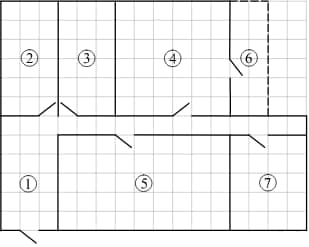
\includegraphics[align=t, width=0.5\linewidth]{\picpath/prob_2.2_1}
		\end{center}
		%2
		\item Краска продаётся в банках по \( 3 \) л. Сколько банок краски требуется купить, чтобы покрасить потолок в гостиной?
			\foranswer
		%3
		\item Найдите площадь, которую занимают детская и балкон. Ответ дайте в квадратных метрах.
		\foranswer
		%4
		\item Найдите расстояние между противоположными углами детской комнаты в метрах. Ответ запишите в виде \( \dfrac{d}{\sqrt{2}} \).
		%5
		\item 
			Хозяин квартиры планирует установить в квартире счётчик. Он рассматривает два варианта: однотарифный или двухтарифный счётчики. Цены на оборудование и стоимость его установки, данные о потребляемой мощности, и тарифах оплаты даны в таблице.
			Обдумав оба варианта, хозяин решил установить двухтарифный электросчётчик. Через сколько дней непрерывного использования электричества экономия от использования двухтарифного счётчика вместо однотарифного компенсирует разность в стоимости установки двухтарифного счётчика и однотарифного?
			\foranswer
		\gapwidth
		\begin{center}
			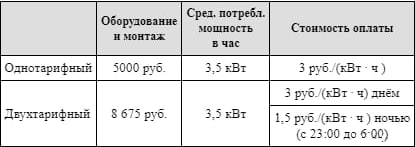
\includegraphics[align=t, width=0.8\linewidth]{\picpath/prob_2.2_2}
		\end{center}
		%6
		\item Найдите значение выражения: \( 2,5\cdot3,5-0,35 \)
		\foranswer
		%7
		\item Известно, что \( 0<a<1 \). Выберите наименьшее из чисел. В ответе укажите номер правильного ответа.
		\begin{tasks}(1)
			\task \( a^2 \)
			\task \( a^3 \)
			\task \( -a \)
			\task \( \dfrac{1}{a} \)
		\end{tasks}
		\foranswer
		%8
		\item Найдите значение выражения \( \sqrt{7\cdot3^4}\cdot\sqrt{7\cdot2^2} \).
		\foranswer
		%9
		\item Решите уравнение \( (x+2)^2+(x-3)^2=2x^2 \)
		\foranswer
		\hphantom{Часть 1}
		%10
		\item Определите вероятность того, что при бросании игрального кубика (правильной кости) выпадет нечетное число очков.
		\foranswer
		%11
		\item На одном из рисунков изображен график функции \( y=x^2-2x+3 \). Укажите номер этого рисунка.
		\begin{center}
			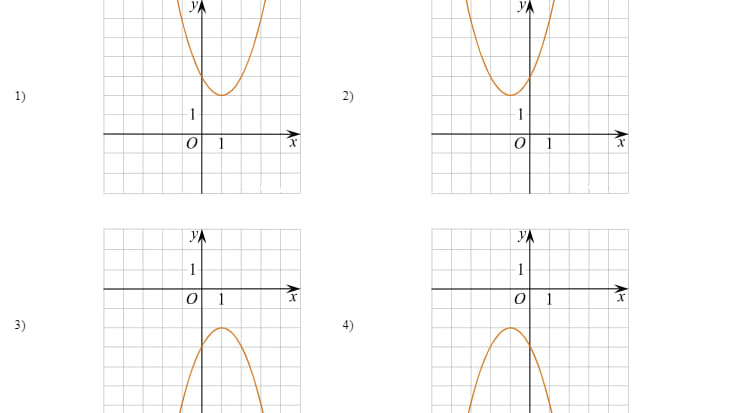
\includegraphics[align=t, width=0.8\linewidth]{\picpath/prob_2.2_4}
		\end{center}
		\foranswer
		%12
		\item Площадь четырёхугольника можно вычислить по формуле \\ \( S=\dfrac{d_1d_2\sin\alpha}{2} \),  где \( d_1 \) и \( d_2 \) --- длины диагоналей четырёхугольника, \( \alpha \) --- угол между диагоналями. Пользуясь этой формулой, найдите длину диагонали \( d_2 \), если \( d_1=6 \), \( \sin\alpha=\dfrac{1}{11} \), а \( S=3 \).
		\foranswer
			\end{listofex}
		\newpage
		\begin{listofex}[resume]
		%13
		\item На каком рисунке изображено множество решений неравенства\\ \( (2x-5)(x+3)\ge0 \)? В ответе укажите номер правильного варианта.
		\begin{center}
			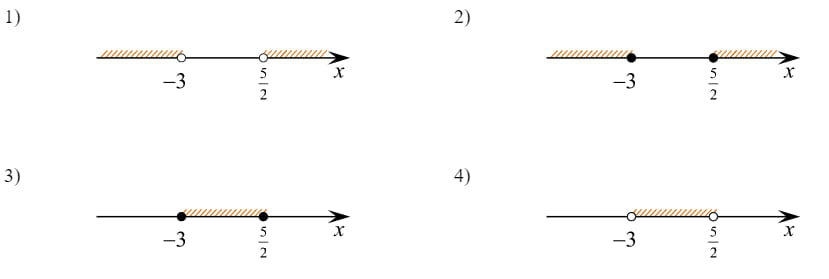
\includegraphics[align=t, width=0.9\linewidth]{\picpath/prob_2.2_6}
		\end{center}
		\foranswer
		%14
		\item Камень бросают в глубокое ущелье. При этом в первую секунду он пролетает \( 15 \) метров, а в каждую следующую секунду на \( 10 \) метров больше, чем в предыдущую, до тех пор, пока не достигнет дна ущелья. Сколько метров пролетит камень за первые четыре секунды?
		\foranswer
		%15
		\item \begin{minipage}[t]{\bodywidth}
			В равнобедренной трапеции известна высота, меньшее основание и угол при основании. Найдите большее основание.
			\foranswer
		\end{minipage}
		\gapwidth
		\begin{minipage}[t]{\picwidth}
			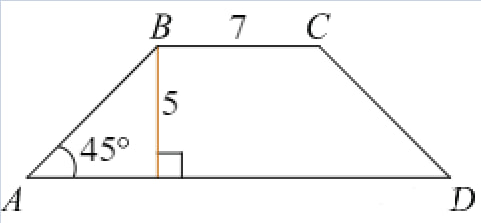
\includegraphics[align=t, width=\linewidth]{\picpath/prob_2.2_8}
		\end{minipage}
		%16
		\item \begin{minipage}[t]{\bodywidth}
			Найдите \( \angle DEF \), если градусные меры дуг \( DE \) и \( EF \) равны \( 150\degree \) и \( 68\degree \) соответственно.
			\foranswer
		\end{minipage}
		\gapwidth
		\begin{minipage}[t]{\picwidth}
			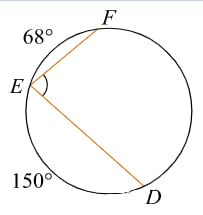
\includegraphics[align=t, width=\linewidth]{\picpath/prob_2.2_10}
		\end{minipage}
		%17
		\item \begin{minipage}[t]{\bodywidth}
		В треугольнике \( ABC \) \( DE \) --- средняя линия. Площадь треугольника \( CDE \) равна \( 9 \). Найдите площадь треугольника \( ABC \).
			\foranswer
		\end{minipage}
		\gapwidth
		\begin{minipage}[t]{\picwidth}
			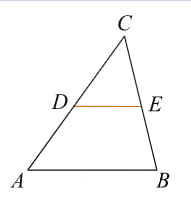
\includegraphics[align=t, width=\linewidth]{\picpath/prob_2.2_11}
		\end{minipage}
		%18
		\item \begin{minipage}[t]{\bodywidth}
			На клетчатой бумаге с размером клетки \( 1\times1 \) изображён треугольник. Найдите его площадь.
			\foranswer
		\end{minipage}
		\gapwidth
		\begin{minipage}[t]{\picwidth}
			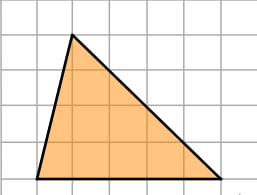
\includegraphics[align=t, width=\linewidth]{\picpath/prob_2.2_13}
		\end{minipage}
		%19
		\item Какие из следующих утверждений верны?
		\begin{tasks}(1)
			\task Через точку, не лежащую на данной прямой, можно провести прямую, параллельную этой
			 прямой.
			 \task Треугольник со сторонами \( 1 \), \( 2 \), \( 4 \) существует.
			 \task В любом параллелограмме есть два равных угла.
		\end{tasks}
		\foranswer
		\title{Часть 2}
		%20
		\item Сократите дробь \( \dfrac{75^n}{5^{2n-1}\cdot3^{n-2}} \)
		%21
		\item Теплоход проходит по течению реки до пункта назначения \( 280 \) км и после стоянки возвращается в пункт отправления. Найдите скорость теплохода в неподвижной воде, если скорость течения равна \( 4 \) км/ч, стоянка длится \( 15 \) часов, а в пункт отправления теплоход возвращается через \( 39 \) часов после отплытия из него.
		%22
		\item Постройте график функции \( y=\dfrac{(x^2+2,25)(x-1)}{1-x} \) и определите, при каких значениях \( k \) прямая \( y=kx \) имеет с графиком ровно одну общую точку.
		%23
		\item Основания трапеции равны \( 16 \) и \( 34 \). Найдите отрезок, соединяющий середины диагоналей трапеции.
		%24
		\item В параллелограмме \( ABCD \) проведены высоты \( BH \) и \( BE \) к сторонам \( AD \) и \( CD \) соответственно, при этом \( BH=BE \). Докажите, что \( ABCD \) --- ромб.
		%25
		\item Основание \( AC \) равнобедренного треугольника \( ABC \) равно \( 10 \). Окружность радиуса \( 7,5 \) \( \, \) с центром вне этого треугольника касается продолжения боковых сторон треугольника и касается основания \( AC \) в его середине. Найдите радиус окружности, вписанной в треугольник \( ABC \).
	\end{listofex}
\end{training}
%END_FOLD

%BEGIN_FOLD % ====>>_____ Вариант 2 _____<<====
\begin{training}[2]
	\title{Часть 1}
	\begin{listofex}
		%1
		\item
		Длина зонта в сложенном виде равна \( 27 \) см и складывается из длины ручки (рис. \( 3 \)) и трети длины спицы (зонт в три сложения). Найдите длину спицы, если длина ручки зонта равна \( 6,8 \) см.\\\\
		Две подруги Оля и Аня задумались о том, как рассчитать площадь поверхности зонта.\\
		На первый взгляд зонт кажется круглым, а его купол напоминает часть сферы (сферический сегмент). Но если присмотреться, то видно, что купол зонта состоит из двенадцати отдельных клиньев, натянутых на каркас из двенадцати спиц (рис. \( 1 \)). Сферическая форма в раскрытом состоянии достигается за счёт гибкости спиц и эластичности ткани, из которой изготовлен зонт.\\
		Оля и Аня сумели измерить расстояние между концами соседних спиц \( a \). Оно оказалось равно \( 28 \) см. Высота купола зонта \( h \) (рис. \( 2 \)) оказалась равна \( 27 \) см, а расстояние \( d \) между концами спиц, образующих дугу окружности, проходящей через вершину зонта, --- ровно \( 108 \) см.
			\foranswer
		\gapwidth
		\begin{center}
			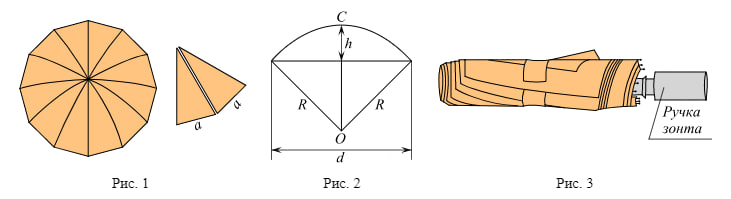
\includegraphics[align=t, width=\linewidth]{\picpath/prob_2.2_3}
		\end{center}
		\foranswer
		%2
		\item
		Поскольку зонт сшит из треугольников, рассуждала Оля, площадь его поверхности можно найти как сумму площадей треугольников. Вычислите площадь поверхности зонта методом Оли, если высота каждого равнобедренного треугольника, проведённая к основанию, равна \( 59 \) см. Ответ дайте в квадратных сантиметрах с округлением до десятков.
		\foranswer
		
		\newpage
		\hphantom{Часть 1}
		%3
		\item Аня предположила, что купол зонта имеет форму сферического сегмента. Вычислите радиус \( R \) сферы купола, зная, что \( OC=R \) (рис. \( 2 \)). Ответ дайте в сантиметрах.
		\foranswer
		%4
		\item Аня нашла площадь купола зонта как площадь поверхности сферического сегмента по формуле \( S=2\pi Rh \), где \( R \) --- радиус сферы, a \( h \) --- высота сегмента. Рассчитайте площадь поверхности купола способом Ани. Число \( \pi \)  округлите до \( 3,14 \). Ответ дайте в квадратных сантиметрах с округлением до целого.
		\foranswer
		%5
		\item Рулон ткани имеет длину \( 20 \) м и ширину \( 90 \) см. На фабрике из этого рулона были вырезаны треугольные клинья для \( 15 \) зонтов, таких же, как зонт, который был у Оли и Ани. Каждый треугольник с учётом припуска на швы имеет площадь \( 850 \) кв. см. Оставшаяся ткань пошла в обрезки. Сколько процентов ткани рулона пошло в обрезки?
		\foranswer
		%6
		\item Найдите значение выражения: \( \dfrac{11}{4,4\cdot2,5} \).
		\foranswer
		%7
		\item Какое из данных чисел принадлежит промежутку \( [7;8] \)? В ответ укажите номер правильного варианта.
		\begin{tasks}(1)
			\task \( \sqrt{7} \)
			\task \( \sqrt{8} \)
			\task \( \sqrt{48} \)
			\task \( \sqrt{56} \)
		\end{tasks}
		\foranswer
		%8
		\item Найдите значение выражения \( (4+\sqrt{5})^2+(4-\sqrt{5})^2 \)
		\foranswer
		\newpage
		%9
		\item Решите систему уравнений: \( \left\{
		\begin{array}{l}
			3x-y=-1,\\
			-x+2y=7
		\end{array}
		\right. \) В ответ запишите \( x+y \).
		\foranswer
		%10
		\item Определите вероятность того, что при бросании игрального кубика (правильной кости) выпадет нечетное число очков.
		\foranswer
		%11
		\item График какой из приведённых ниже функций изображён на рисунке?
		\begin{center}
			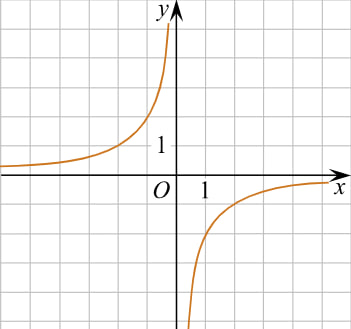
\includegraphics[align=t, width=0.5\linewidth]{\picpath/prob_2.2_5}
		\end{center}
		\begin{tasks}(4)
			\task \( y=-\dfrac{2}{x} \)
			\task \( y=\dfrac{2}{x} \)
			\task \( y=-\dfrac{1}{2x} \)
			\task \( y=\dfrac{1}{2x} \)
		\end{tasks}
		\foranswer
		%12
		\item Площадь четырёхугольника можно вычислить по формуле \\ \( S=\dfrac{d_1d_2\sin\alpha}{2} \),  где \( d_1 \) и \( d_2 \) --- длины диагоналей четырёхугольника, \( \alpha \) --- угол между диагоналями. Пользуясь этой формулой, найдите длину диагонали \( d_2 \), если \( d_1=6 \), \( \sin\alpha=\dfrac{1}{11} \), а \( S=3 \).
		\foranswer
		%13
		\item Решите неравенство \( x^2-4x<0 \). В ответ укажите номер правильного ответа.
		\begin{tasks}(1)
			\task \( [0;4] \)
			\task \( (-\infty;0)\cup(4;+\infty) \)
			\task \( (0;4) \)
			\task \( (-\infty;0]\cup[4;+\infty) \)
		\end{tasks}
		\foranswer
		%14
		\item У Светы есть попрыгунчик (каучуковый шарик). Она со всей силы бросила его об асфальт. После первого отскока попрыгунчик подлетел на высоту \( 560 \) см, а после каждого следующего отскока от асфальта подлетал на высоту в два раза меньше предыдущей. После какого по счёту отскока высота, на которую подлетит попрыгунчик, станет меньше \( 20 \) см?
		\foranswer
		%15
		\item
		\begin{minipage}[t]{\bodywidth}
			Тангенс острого угла прямоугольной трапеции равен \( \dfrac{5}{6} \).  Найдите её большее основание, если меньшее основание равно высоте и равно \( 15 \).
			\foranswer
		\end{minipage}
		\gapwidth
		\begin{minipage}[t]{\picwidth}
			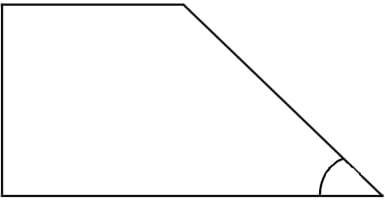
\includegraphics[align=t, width=\linewidth]{\picpath/prob_2.2_7}
		\end{minipage}
		%16
		\item 
		\begin{minipage}[t]{\bodywidth}
			Прямая касается окружности в точке \( K \). Точка \( O \) --- центр окружности. Хорда \( KM \) образует с касательной угол, равный \( 75\degree \). Найдите величину угла \( OMK \). Ответ дайте в градусах.
			\foranswer
		\end{minipage}
		\gapwidth
		\begin{minipage}[t]{\picwidth}
			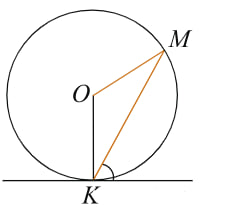
\includegraphics[align=t, width=\linewidth]{\picpath/prob_2.2_9}
		\end{minipage}
		%17
		\item Основания трапеции равны \( 18 \) и \( 12 \), одна из боковых сторон равна \( 6 \), а синус угла между ней и одним из оснований равен \( \dfrac{1}{3} \).  Найдите площадь трапеции.
		\foranswer
		%18
		\item \begin{minipage}[t]{\bodywidth}
			На рисунке изображен параллелограмм \( ABCD \). Используя рисунок, найдите \( \sin\angle HBA \).
			\foranswer
		\end{minipage}
		\gapwidth
		\begin{minipage}[t]{\picwidth}
			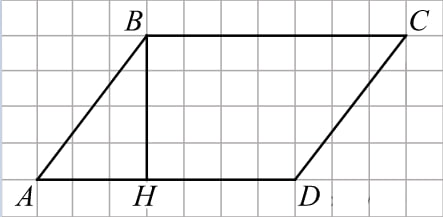
\includegraphics[align=t, width=\linewidth]{\picpath/prob_2.2_12}
		\end{minipage}
		%19
		\item Какие из следующих утверждений верны?
		\begin{tasks}(1)
			\task Любые два прямоугольных треугольника подобны.
			\task Если катет и гипотенуза прямоугольного треугольника равны соответственно \( 6 \) и \( 10 \), то второй катет этого треугольника равен \( 8 \).
			\task Стороны треугольника пропорциональны косинусам противолежащих углов.
			\task Квадрат любой стороны треугольника равен сумме квадратов двух других сторон без удвоенного произведения этих сторон на косинус угла между ними.
		\end{tasks}
		\foranswer
		\title{Часть 2}
		%20
		\item Решите уравнение \( (x^2-9)^2+(x^2-2x-15)^2=0 \)
		%21
		\item При смешивании первого раствора кислоты, концентрация которого \( 20\% \), и второго раствора этой же кислоты, концентрация которого \( 50\% \), получили раствор, содержащий \( 30\% \) кислоты. В каком отношении были взяты первый и второй растворы?
		%22
		\item Постройте график функции
		\[y= \left\{
		\begin{array}{l}
			x-3, \quad x<3,\\
			-1,5x+4,5,\quad 3\le x\le4,\\
			1,5x-7,5, \quad x>4,
		\end{array}
		\right.\]
		и определите, при каких значениях \( m \) прямая \( y=m \) имеет с графиком ровно две общие точки.
		%23
		\item Основания трапеции равны \( 16 \) и \( 34 \). Найдите отрезок, соединяющий середины диагоналей трапеции.
		%24
		\item На медиане \( KF \) треугольника \( MKP \) отмечена точка \( E \). Докажите, что если \( EM=EP \), то \( KM=KP \).
		%25
		\item Основание \( AC \) равнобедренного треугольника \( ABC \) равно \( 10 \). Окружность радиуса \( 7,5 \) \( \, \) с центром вне этого треугольника касается продолжения боковых сторон треугольника и касается основания \( AC \) в его середине. Найдите радиус окружности, вписанной в треугольник \( ABC \).
	\end{listofex}
\end{training}
%END_FOLD